\section{非线性系统}

\subsection{非线性系统概述}

\subsubsection{非线性系统的定义}

\textbf{非线性系统}是指不满足叠加原理的系统,其数学模型为非线性微分方程。

\begin{minipage}[t]{0.48\textwidth}
\textbf{线性系统 vs 非线性系统:}

\textbf{线性系统:}
\begin{itemize}
    \item 满足叠加原理(齐次性和可加性)
    \item 数学模型:线性微分方程
    \item 解法:拉普拉斯变换、传递函数等
    \item 频率响应:可用频域方法分析
\end{itemize}

\textbf{非线性系统:}
\begin{itemize}
    \item 不满足叠加原理
    \item 数学模型:非线性微分方程
    \item 解法:相平面法、描述函数法等
    \item 响应:依赖于输入幅值和初始条件
\end{itemize}

\vspace{0.3cm}
\textbf{典型非线性特性:}

\begin{enumerate}
    \item \textbf{饱和特性}:放大器、执行机构的幅值限制
    \item \textbf{死区特性}:齿轮间隙、阈值检测
    \item \textbf{间隙特性}:机械传动中的空程
    \item \textbf{继电特性}:开关、继电器
    \item \textbf{摩擦特性}:库伦摩擦、粘性摩擦
\end{enumerate}
\end{minipage}\hfill
\begin{minipage}[t]{0.48\textwidth}
\vspace{0pt}
\textbf{典型非线性环节图示:}

\begin{center}
\begin{tikzpicture}[scale=0.65]
% 饱和特性
\begin{scope}[shift={(0,6)}]
\draw[->] (-2,0) -- (2,0) node[right] {\tiny $x$};
\draw[->] (0,-1.5) -- (0,1.5) node[above] {\tiny $y$};
\draw[blue, thick] (-2,-1) -- (-1,-1) -- (1,1) -- (2,1);
\node[below] at (0,-1.8) {\small 饱和};
\draw[dashed, red] (-1,0) -- (-1,-1);
\draw[dashed, red] (1,0) -- (1,1);
\end{scope}

% 死区特性
\begin{scope}[shift={(5,6)}]
\draw[->] (-2,0) -- (2,0) node[right] {\tiny $x$};
\draw[->] (0,-1.5) -- (0,1.5) node[above] {\tiny $y$};
\draw[blue, thick] (-2,-1.5) -- (-0.5,0) -- (0.5,0) -- (2,1.5);
\node[below] at (0,-1.8) {\small 死区};
\draw[dashed, red] (-0.5,0) -- (-0.5,-0.3);
\draw[dashed, red] (0.5,0) -- (0.5,-0.3);
\end{scope}

% 间隙特性
\begin{scope}[shift={(0,2)}]
\draw[->] (-2,0) -- (2,0) node[right] {\tiny $x$};
\draw[->] (0,-1.5) -- (0,1.5) node[above] {\tiny $y$};
\draw[blue, thick] (-2,-1.2) -- (-0.4,0.4);
\draw[blue, thick] (0.4,-0.4) -- (2,1.2);
\draw[blue, thick, <->] (-0.4,0.4) -- (0.4,-0.4);
\node[below] at (0,-1.8) {\small 间隙};
\end{scope}

% 继电特性
\begin{scope}[shift={(5,2)}]
\draw[->] (-2,0) -- (2,0) node[right] {\tiny $x$};
\draw[->] (0,-1.5) -- (0,1.5) node[above] {\tiny $y$};
\draw[blue, thick] (-2,1) -- (0,1);
\draw[blue, thick] (0,-1) -- (2,-1);
\draw[blue, thick, dashed] (0,1) -- (0,-1);
\node[below] at (0,-1.8) {\small 继电};
\node[left] at (0,1) {\tiny $M$};
\node[left] at (0,-1) {\tiny $-M$};
\end{scope}

% 摩擦特性
\begin{scope}[shift={(2.5,-1.5)}]
\draw[->] (-2,0) -- (2,0) node[right] {\tiny $\dot{x}$};
\draw[->] (0,-1.5) -- (0,1.5) node[above] {\tiny $F$};
\draw[blue, thick] (-2,-0.8) -- (-0.3,-0.5) -- (0.3,0.5) -- (2,0.8);
\node[below] at (0,-1.8) {\small 摩擦};
\draw[dashed, red] (-0.3,0) -- (-0.3,-0.5);
\draw[dashed, red] (0.3,0) -- (0.3,0.5);
\end{scope}
\end{tikzpicture}
\end{center}
\end{minipage}

\subsubsection{非线性系统的特点}

\begin{enumerate}
    \item \textbf{不满足叠加原理}:输出不与输入成线性关系
    \item \textbf{稳定性复杂}:可能存在多个平衡点,稳定性依赖于初始条件
    \item \textbf{极限环}:自激振荡,振幅和频率由系统参数决定
    \item \textbf{跳变现象}:参数变化时系统响应突变
    \item \textbf{分岔现象}:系统行为质的变化
    \item \textbf{混沌}:对初始条件极度敏感的复杂运动
\end{enumerate}

\subsection{相平面法}

相平面法是分析二阶非线性系统的图解方法,通过绘制相轨迹来研究系统的动态行为。

\subsubsection{相平面与相轨迹}

\begin{minipage}[t]{0.52\textwidth}
\textbf{基本概念:}

\textbf{1. 状态空间表示}

二阶系统:
\begin{align*}
\ddot{x} &= f(x, \dot{x}) \\
\text{令:} x_1 &= x, \quad x_2 = \dot{x} \\
\dot{x}_1 &= x_2 \\
\dot{x}_2 &= f(x_1, x_2)
\end{align*}

\textbf{2. 相平面}

以 $x$ 为横轴,$\dot{x}$ 为纵轴构成的平面。

\textbf{3. 相轨迹}

系统在相平面上的运动轨迹,表示系统状态随时间的变化。

\textbf{4. 奇点(平衡点)}

满足 $\dot{x} = 0$ 和 $\ddot{x} = 0$ 的点。

\vspace{0.3cm}
\textbf{奇点分类:}

\begin{itemize}
    \item \textbf{稳定焦点}:螺旋收敛到奇点
    \item \textbf{不稳定焦点}:螺旋发散
    \item \textbf{稳定节点}:直接收敛到奇点
    \item \textbf{不稳定节点}:直接发散
    \item \textbf{鞍点}:沿某方向稳定,沿另一方向不稳定
    \item \textbf{中心}:封闭的椭圆轨迹(等幅振荡)
\end{itemize}
\end{minipage}\hfill
\begin{minipage}[t]{0.45\textwidth}
\vspace{0pt}
\textbf{典型奇点的相轨迹:}

\begin{center}
\begin{tikzpicture}[scale=0.5]
% 稳定焦点
\begin{scope}[shift={(0,6)}]
\draw[->] (-1.5,0) -- (1.5,0) node[right] {\tiny $x$};
\draw[->] (0,-1.5) -- (0,1.5) node[above] {\tiny $\dot{x}$};
\draw[blue, thick, domain=0:10*pi, samples=200, smooth] 
    plot ({0.8*exp(-0.1*\x)*cos(\x r)}, {0.8*exp(-0.1*\x)*sin(\x r)});
\fill (0,0) circle (2pt);
\node[below] at (0,-1.8) {\small 稳定焦点};
\end{scope}

% 不稳定节点
\begin{scope}[shift={(5,6)}]
\draw[->] (-1.5,0) -- (1.5,0) node[right] {\tiny $x$};
\draw[->] (0,-1.5) -- (0,1.5) node[above] {\tiny $\dot{x}$};
\draw[blue, thick, ->] (0.2,0.1) -- (1,0.5);
\draw[blue, thick, ->] (0.1,0.2) -- (0.5,1);
\draw[blue, thick, ->] (-0.2,-0.1) -- (-1,-0.5);
\draw[blue, thick, ->] (-0.1,-0.2) -- (-0.5,-1);
\fill (0,0) circle (2pt);
\node[below] at (0,-1.8) {\small 不稳定节点};
\end{scope}

% 鞍点
\begin{scope}[shift={(0,2)}]
\draw[->] (-1.5,0) -- (1.5,0) node[right] {\tiny $x$};
\draw[->] (0,-1.5) -- (0,1.5) node[above] {\tiny $\dot{x}$};
\draw[blue, thick, ->] (-1,-0.3) -- (-0.1,-0.05);
\draw[blue, thick, ->] (1,0.3) -- (0.1,0.05);
\draw[blue, thick, ->] (-0.3,-1) -- (-1.2,-0.5);
\draw[blue, thick, ->] (0.3,1) -- (1.2,0.5);
\fill (0,0) circle (2pt);
\node[below] at (0,-1.8) {\small 鞍点};
\end{scope}

% 中心
\begin{scope}[shift={(5,2)}]
\draw[->] (-1.5,0) -- (1.5,0) node[right] {\tiny $x$};
\draw[->] (0,-1.5) -- (0,1.5) node[above] {\tiny $\dot{x}$};
\draw[blue, thick] (0,0) circle (0.5);
\draw[blue, thick] (0,0) circle (1);
\fill (0,0) circle (2pt);
\node[below] at (0,-1.8) {\small 中心};
\end{scope}
\end{tikzpicture}
\end{center}

\textbf{相轨迹的性质:}

\begin{itemize}
    \item 不同轨迹不相交(除奇点外)
    \item 轨迹方向由 $\dot{x}$ 的符号决定
    \item 封闭轨迹对应周期运动
    \item 螺旋轨迹对应振荡运动
\end{itemize}
\end{minipage}

\subsubsection{等倾线法}

\textbf{等倾线}是相平面上相轨迹斜率相等的点的轨迹。

\textbf{方法:}

1. 计算相轨迹斜率:
\begin{align*}
\frac{d\dot{x}}{dx} = \frac{\ddot{x}}{\dot{x}} = \frac{f(x, \dot{x})}{\dot{x}}
\end{align*}

2. 令斜率为常数 $\alpha$,得等倾线方程:
\begin{align*}
\frac{f(x, \dot{x})}{\dot{x}} = \alpha \implies f(x, \dot{x}) = \alpha \dot{x}
\end{align*}

3. 绘制不同 $\alpha$ 值对应的等倾线

4. 从初始点开始,沿等倾线指示的方向绘制相轨迹

\vspace{0.3cm}
\textbf{例题:}二阶线性系统 $\ddot{x} + 2\zeta\omega_n\dot{x} + \omega_n^2 x = 0$,$\omega_n = 1$,$\zeta = 0.5$,用相平面法分析。

\textit{解:}

\textbf{1. 建立相平面方程}
\begin{align*}
\dot{x}_2 &= -\omega_n^2 x_1 - 2\zeta\omega_n x_2 = -x_1 - x_2
\end{align*}

\textbf{2. 奇点}

$(0, 0)$ 是唯一的奇点。

\textbf{3. 判断奇点类型}

特征方程:$\lambda^2 + 2\zeta\omega_n\lambda + \omega_n^2 = 0$

$\lambda = -0.5 \pm 0.866j$(共轭复根,实部为负)

结论:\textbf{稳定焦点}

\textbf{4. 相轨迹}

螺旋收敛到原点,表示系统稳定且有振荡。

\subsection{描述函数法}

描述函数法是分析含有非线性环节的闭环系统的近似频域方法。

\subsubsection{描述函数的定义}

对于非线性环节,当输入为正弦信号 $x = A\sin\omega t$ 时,输出一般为非正弦周期信号。

\begin{minipage}[t]{0.52\textwidth}
\textbf{基本假设:}

\begin{enumerate}
    \item 非线性环节的输出可以用傅里叶级数展开
    \item 线性部分对高次谐波有足够的衰减(低通滤波特性)
    \item 只考虑基波分量的作用
\end{enumerate}

\textbf{描述函数定义:}

非线性环节输出的基波分量与输入振幅的复数比:
\begin{align*}
N(A) = \frac{Y_1(A)}{A}
\end{align*}

其中 $Y_1(A)$ 是输出的基波复数幅值。

\vspace{0.3cm}
\textbf{计算方法:}

输出 $y(t)$ 的傅里叶展开:
\begin{align*}
y(t) &= a_0 + \sum_{n=1}^{\infty} (a_n\cos n\omega t + b_n\sin n\omega t) \\
a_n &= \frac{2}{T}\int_0^T y(t)\cos n\omega t \, dt \\
b_n &= \frac{2}{T}\int_0^T y(t)\sin n\omega t \, dt
\end{align*}

基波分量:$Y_1 = \sqrt{a_1^2 + b_1^2}$

相位:$\phi_1 = \arctan(a_1/b_1)$

描述函数:
\begin{align*}
N(A) = \frac{Y_1}{A} e^{j\phi_1}
\end{align*}
\end{minipage}\hfill
\begin{minipage}[t]{0.45\textwidth}
\vspace{0pt}
\textbf{典型非线性环节的描述函数:}

\textbf{1. 饱和特性}

\begin{center}
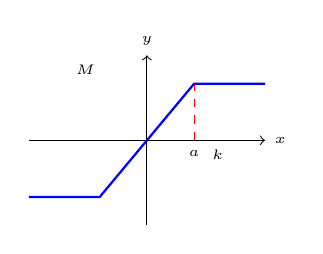
\begin{tikzpicture}[scale=0.6]
\draw[->] (-2.5,0) -- (2.5,0) node[right] {\tiny $x$};
\draw[->] (0,-1.8) -- (0,1.8) node[above] {\tiny $y$};
\draw[blue, thick] (-2.5,-1.2) -- (-1,-1.2) -- (1,1.2) -- (2.5,1.2);
\node at (1.5,-0.3) {\tiny $k$};
\node at (-1.3,1.5) {\tiny $M$};
\draw[dashed, red] (1,0) -- (1,1.2);
\node[below] at (1,0) {\tiny $a$};
\end{tikzpicture}
\end{center}

\begin{align*}
N(A) = \begin{cases}
k & A \leq a \\
\frac{2k}{\pi}\left[\arcsin\frac{a}{A} + \frac{a}{A}\sqrt{1-\left(\frac{a}{A}\right)^2}\right] & A > a
\end{cases}
\end{align*}

其中 $a = M/k$(饱和阈值)

\textbf{2. 死区特性}

\begin{align*}
N(A) = \begin{cases}
0 & A \leq \Delta \\
\frac{k}{\pi}\left[\pi - 2\arcsin\frac{\Delta}{A} - \frac{2\Delta}{A}\sqrt{1-\left(\frac{\Delta}{A}\right)^2}\right] & A > \Delta
\end{cases}
\end{align*}

\textbf{3. 继电特性}

\begin{align*}
N(A) = \frac{4M}{\pi A}
\end{align*}

$M$ 为继电器输出幅值
\end{minipage}

\subsubsection{稳定性分析}

\textbf{闭环系统结构:}

非线性环节 $N(A)$ 串联线性部分 $G(j\omega)$ 构成单位负反馈系统。

\textbf{稳定性判据(类似奈奎斯特判据):}

系统稳定的条件:
\begin{align*}
G(j\omega) \text{曲线不包围点} \left(-\frac{1}{N(A)}\right)
\end{align*}

\textbf{极限环判断:}

极限环存在的条件:
\begin{align*}
G(j\omega_0) = -\frac{1}{N(A_0)}
\end{align*}

此时系统产生频率为 $\omega_0$、幅值为 $A_0$ 的自激振荡。

\vspace{0.3cm}
\textbf{稳定性判断:}

\begin{itemize}
    \item 若 $-1/N(A)$ 曲线在 $G(j\omega)$ 外侧:稳定
    \item 若相交:存在极限环
    \item 极限环稳定性:由交点处曲线的相对位置决定
\end{itemize}

\vspace{0.3cm}
\textbf{例题:}系统含继电特性 $M=1$,线性部分 $G(s) = \frac{K}{s(s+1)}$,$K=2$,判断是否存在极限环。

\textit{解:}

\textbf{1. 继电特性的描述函数}
\begin{align*}
N(A) = \frac{4M}{\pi A} = \frac{4}{\pi A}
\end{align*}

\textbf{2. $-1/N(A)$ 曲线}
\begin{align*}
-\frac{1}{N(A)} = -\frac{\pi A}{4}
\end{align*}

这是实轴上的负半轴,$A$ 从 $0$ 到 $\infty$ 变化时,点从 $0$ 到 $-\infty$ 移动。

\textbf{3. $G(j\omega)$ 曲线}
\begin{align*}
G(j\omega) = \frac{2}{j\omega(1+j\omega)} = \frac{2(1-j\omega)}{\omega^2(1+\omega^2)}
\end{align*}

\textbf{4. 交点判断}

令 $\text{Im}[G(j\omega)] = 0$:$-2/[\omega^2(1+\omega^2)] = 0$ 无解

$G(j\omega)$ 曲线不与实轴负半轴相交 $\implies$ 不存在极限环。

\textbf{结论:}系统不会产生自激振荡。

\subsection{Lyapunov稳定性理论(非线性系统)}

Lyapunov第二方法(直接法)适用于非线性系统的稳定性分析,无需求解微分方程。

\subsubsection{Lyapunov稳定性定义}

考虑非线性系统:
\begin{align*}
\dot{\mathbf{x}} = \mathbf{f}(\mathbf{x}, t)
\end{align*}

假设 $\mathbf{x}_e$ 是平衡点($\mathbf{f}(\mathbf{x}_e, t) = 0$)。

\textbf{稳定性定义:}

\begin{itemize}
    \item \textbf{稳定}:对任意 $\epsilon > 0$,存在 $\delta > 0$,使得当 $\|\mathbf{x}(0) - \mathbf{x}_e\| < \delta$ 时,有 $\|\mathbf{x}(t) - \mathbf{x}_e\| < \epsilon$($t \geq 0$)
    \item \textbf{渐近稳定}:稳定且 $\lim_{t\to\infty} \mathbf{x}(t) = \mathbf{x}_e$
    \item \textbf{全局渐近稳定}:对任意初始条件都渐近稳定
\end{itemize}

\subsubsection{Lyapunov定理}

\textbf{定理(Lyapunov稳定性定理):}

如果存在标量函数 $V(\mathbf{x})$(Lyapunov函数)满足:

\begin{enumerate}
    \item $V(\mathbf{x})$ 连续可微
    \item $V(\mathbf{x}_e) = 0$ 且在 $\mathbf{x} \neq \mathbf{x}_e$ 时 $V(\mathbf{x}) > 0$(正定)
    \item $\dot{V}(\mathbf{x}) = \frac{\partial V}{\partial \mathbf{x}} \cdot \mathbf{f}(\mathbf{x}, t) \leq 0$(半负定)
\end{enumerate}

则平衡点 $\mathbf{x}_e$ 是\textbf{稳定}的。

如果进一步满足:
\begin{enumerate}
    \setcounter{enumi}{3}
    \item $\dot{V}(\mathbf{x}) < 0$($\mathbf{x} \neq \mathbf{x}_e$,负定)
\end{enumerate}

则平衡点 $\mathbf{x}_e$ 是\textbf{渐近稳定}的。

\vspace{0.3cm}
\textbf{Lyapunov函数的构造:}

常用形式(二次型):
\begin{align*}
V(\mathbf{x}) = \mathbf{x}^T \mathbf{P} \mathbf{x}
\end{align*}

其中 $\mathbf{P}$ 是正定对称矩阵。

\vspace{0.3cm}
\textbf{例题:}分析系统 $\dot{x}_1 = x_2$,$\dot{x}_2 = -x_1 - x_2$ 的稳定性。

\textit{解:}

\textbf{1. 确定平衡点}

令 $\dot{x}_1 = \dot{x}_2 = 0$:$x_1 = x_2 = 0$

\textbf{2. 构造Lyapunov函数}

选择:$V(x_1, x_2) = x_1^2 + x_2^2$

\textbf{3. 验证正定性}

$V(0, 0) = 0$ 且 $V(x_1, x_2) > 0$($x_1, x_2$ 不全为零)$\implies$ 正定

\textbf{4. 计算 $\dot{V}$}
\begin{align*}
\dot{V} &= \frac{\partial V}{\partial x_1}\dot{x}_1 + \frac{\partial V}{\partial x_2}\dot{x}_2 \\
&= 2x_1 \cdot x_2 + 2x_2 \cdot (-x_1 - x_2) \\
&= 2x_1 x_2 - 2x_1 x_2 - 2x_2^2 \\
&= -2x_2^2 \leq 0
\end{align*}

$\dot{V} < 0$(除原点外)$\implies$ 负定

\textbf{结论:}原点是\textbf{渐近稳定}的平衡点。

\subsection{总结}

\begin{center}
\begin{tabular}{|l|p{4cm}|p{4cm}|p{3cm}|}
\hline
\textbf{方法} & \textbf{适用范围} & \textbf{优点} & \textbf{缺点} \\
\hline
相平面法 & 二阶系统 & 直观、图形化 & 仅限二阶 \\
\hline
描述函数法 & 含单一非线性环节 & 频域分析、预测极限环 & 近似方法 \\
\hline
Lyapunov法 & 任意阶非线性系统 & 严格、不需求解方程 & 构造函数困难 \\
\hline
\end{tabular}
\end{center}
